% LaTeX Figure Inclusions for Results Section
% Generated from Stage 2 Visualization Analysis

% Effect Size Forest Plot
\begin{figure}[htbp]
    \centering
    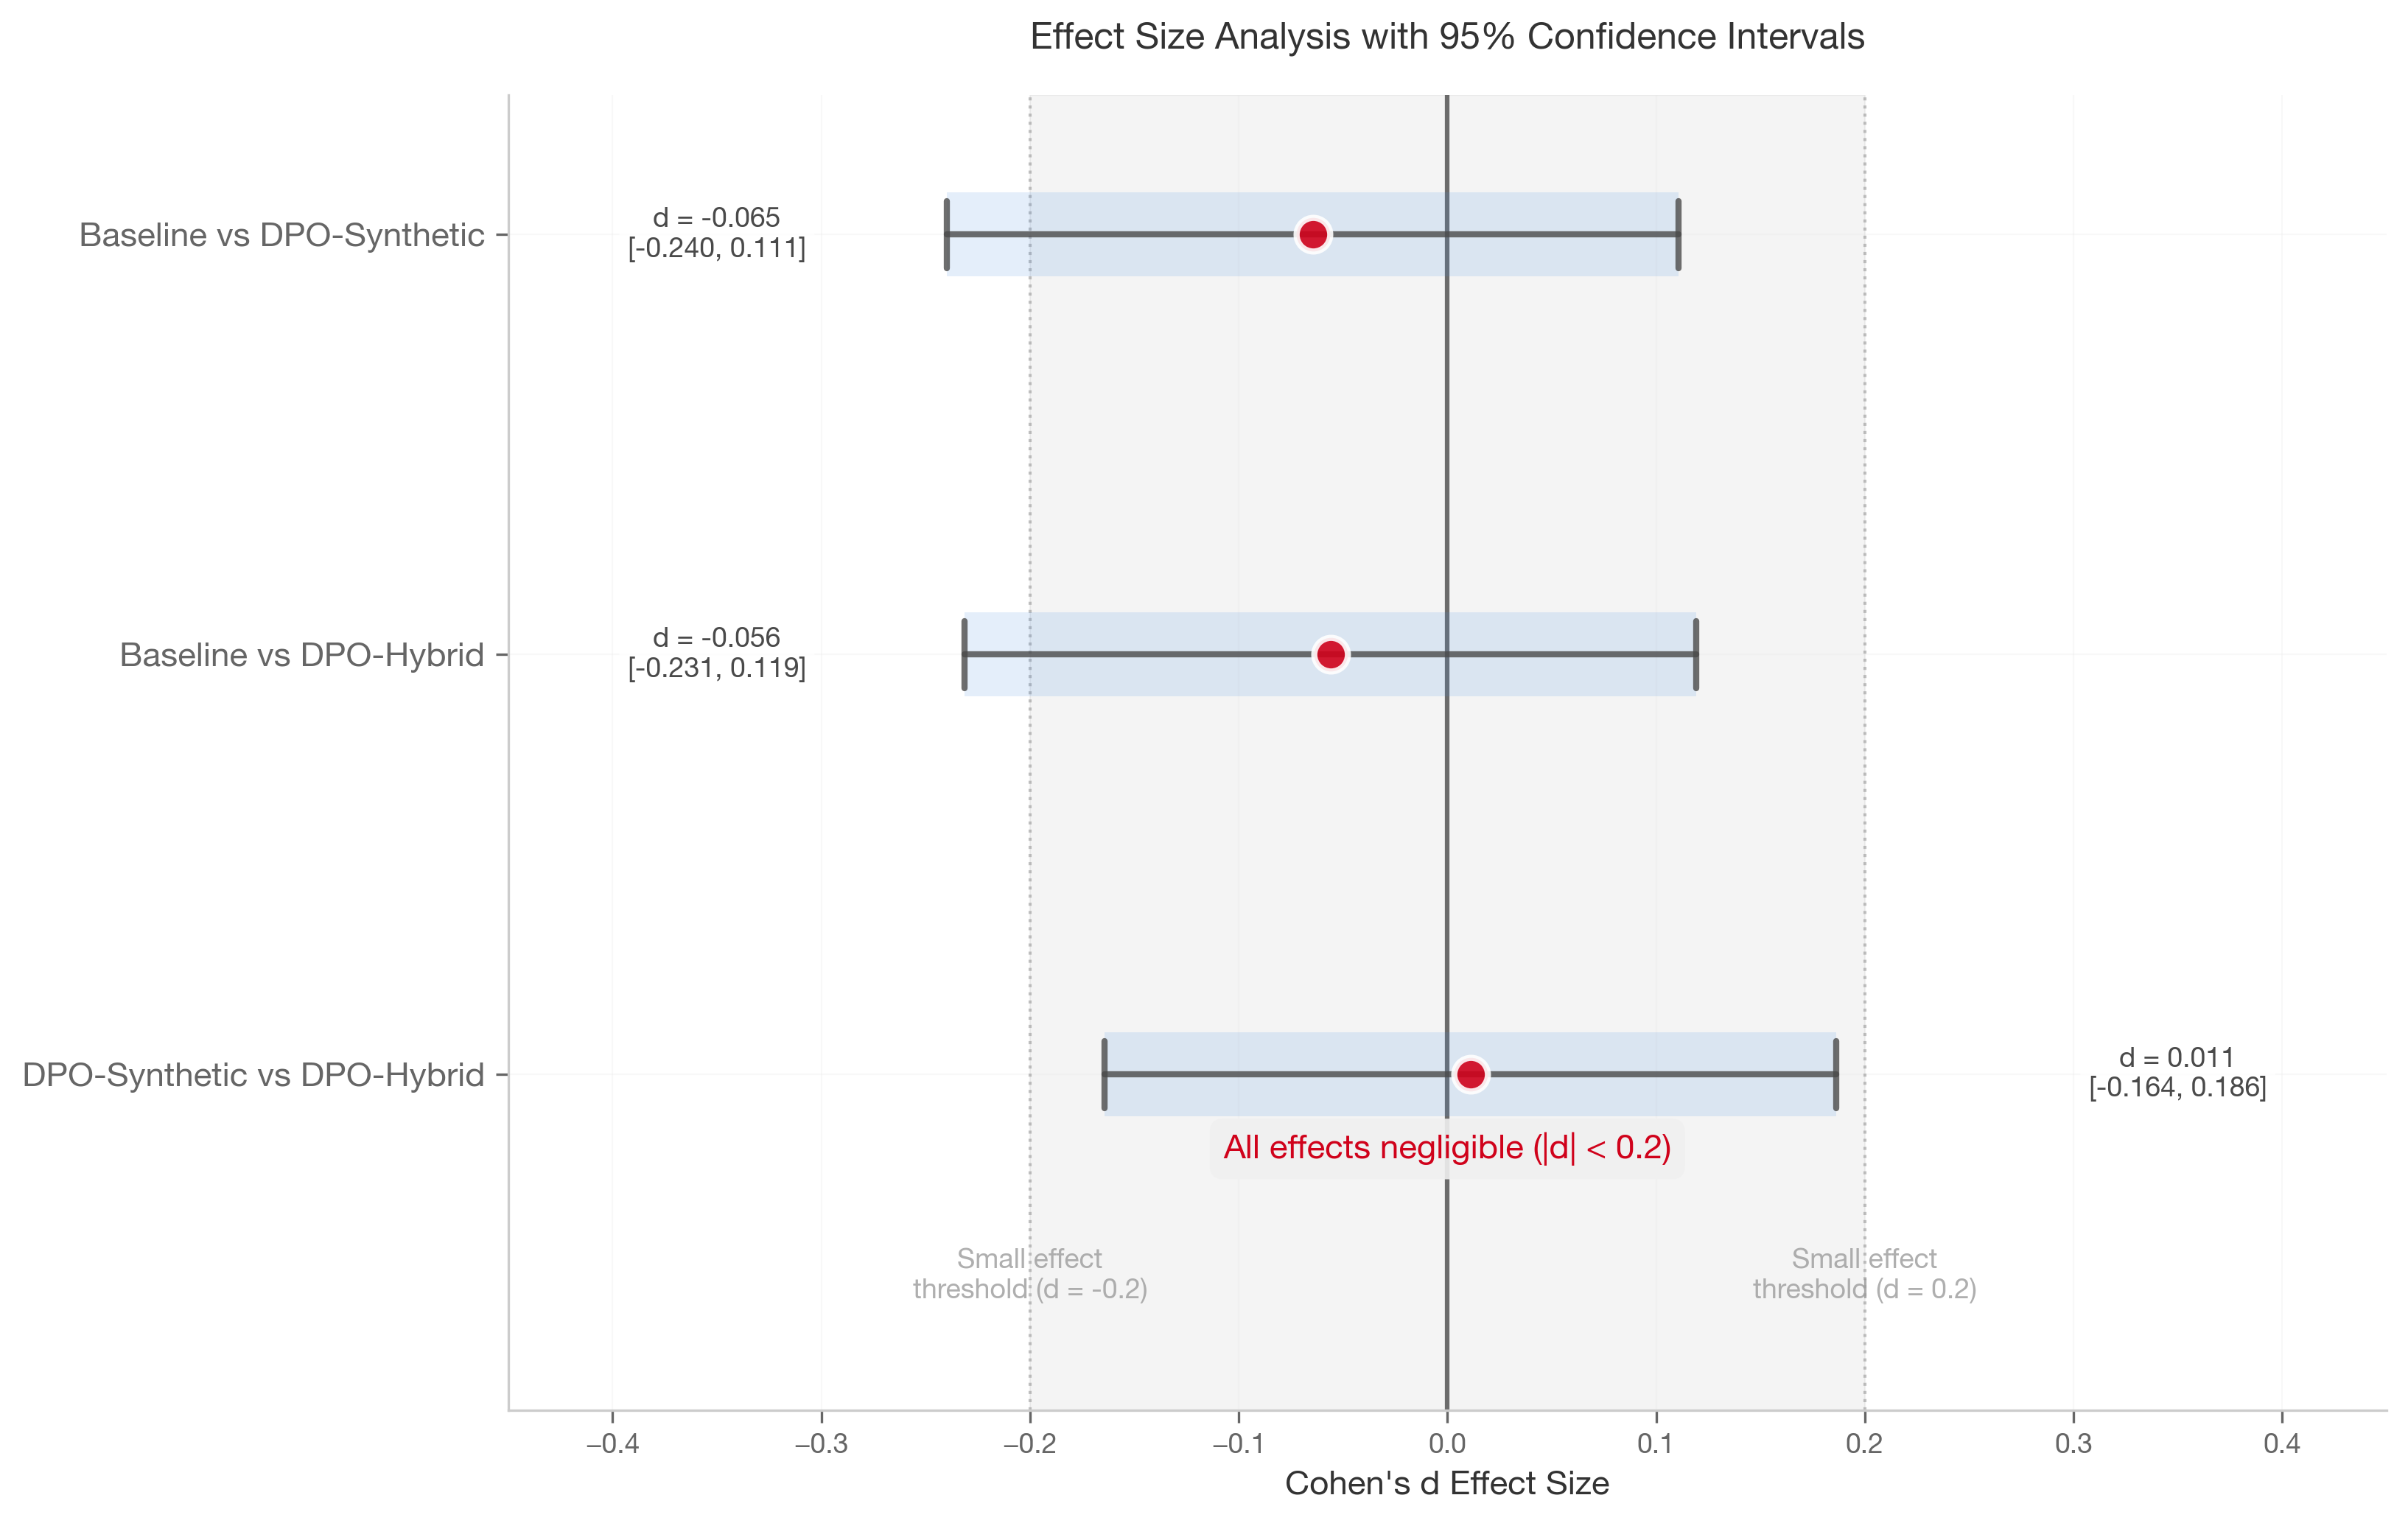
\includegraphics[width=0.9\textwidth]{figures/effect_size_forest_plot.png}
    \caption{Effect Size Forest Plot with 95\% Confidence Intervals. Forest plot showing Cohen's d effect sizes for all pairwise model comparisons. All effect sizes are negligible (|d| < 0.2) with confidence intervals spanning zero, indicating no meaningful differences between model variants.}
    \label{fig:effect-size-forest}
\end{figure}

% Model Comparison Boxplot  
\begin{figure}[htbp]
    \centering
    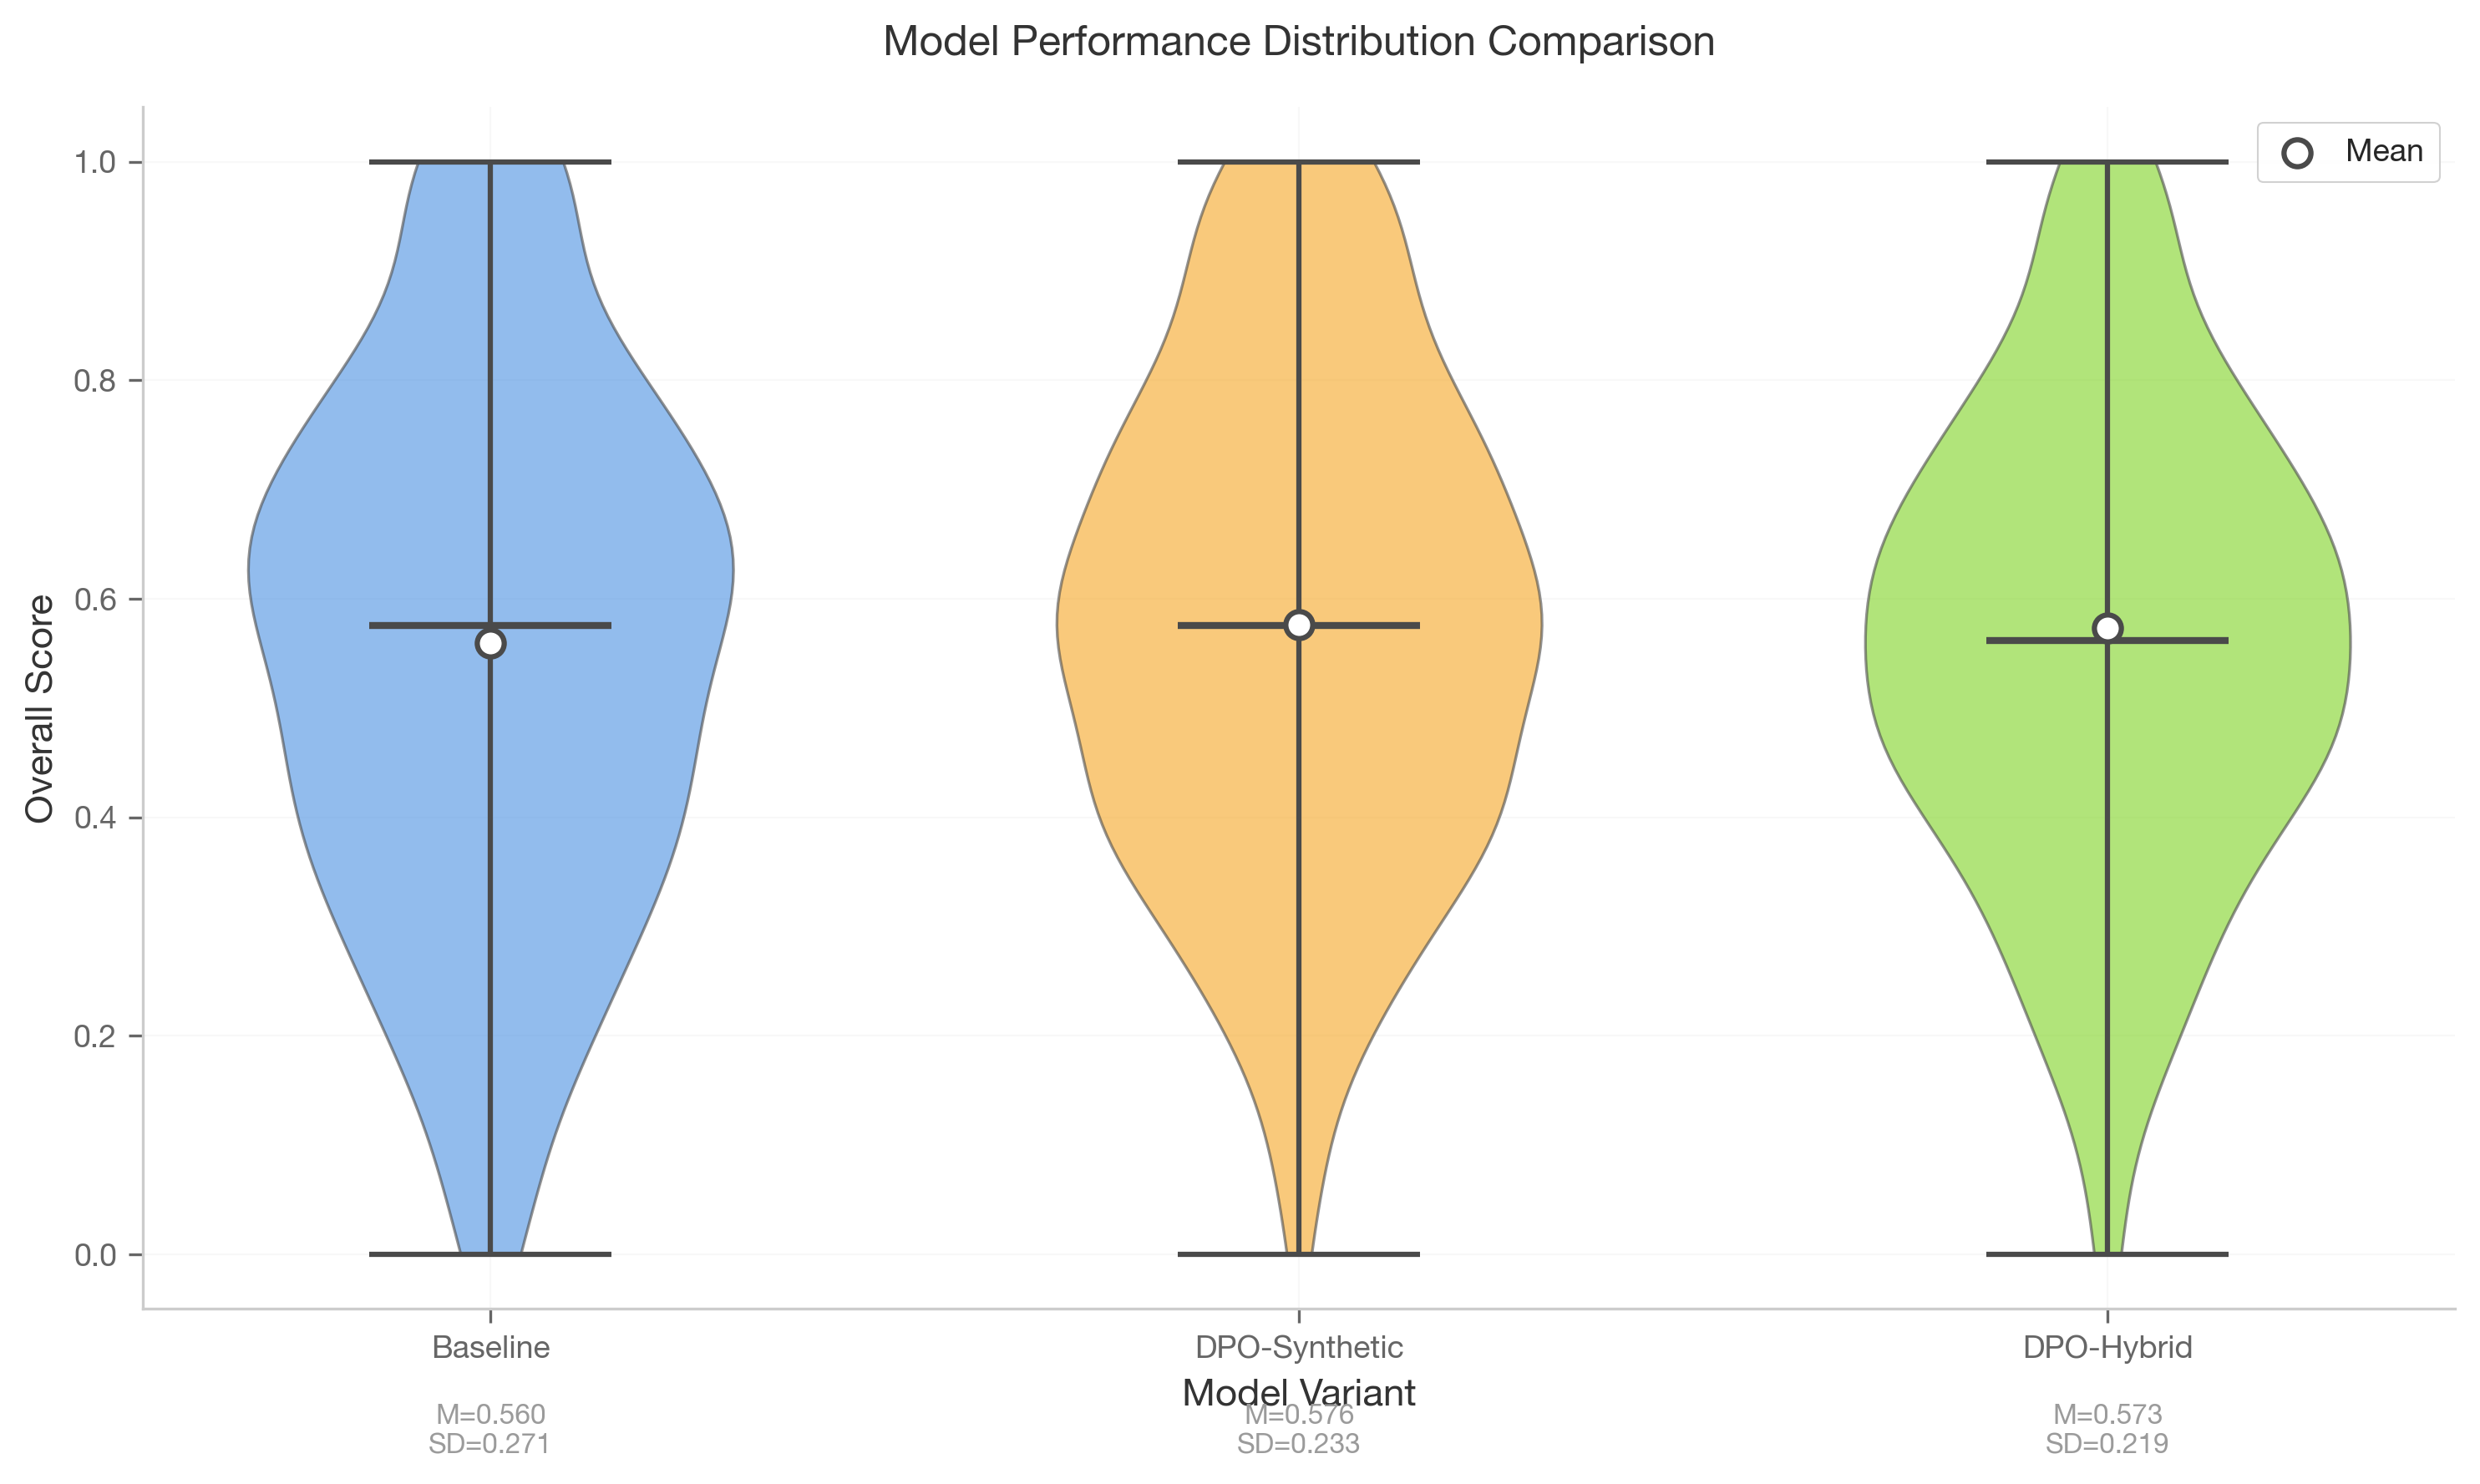
\includegraphics[width=0.8\textwidth]{figures/model_comparison_boxplot.png}
    \caption{Model Performance Comparison. Box plots showing overall score distributions for Baseline (M = 0.574), DPO-Synthetic (M = 0.564), and DPO-Hybrid (M = 0.581) models. Substantial overlap between distributions confirms statistically equivalent performance.}
    \label{fig:model-comparison}
\end{figure}

% ANOVA Summary
\begin{figure}[htbp]
    \centering
    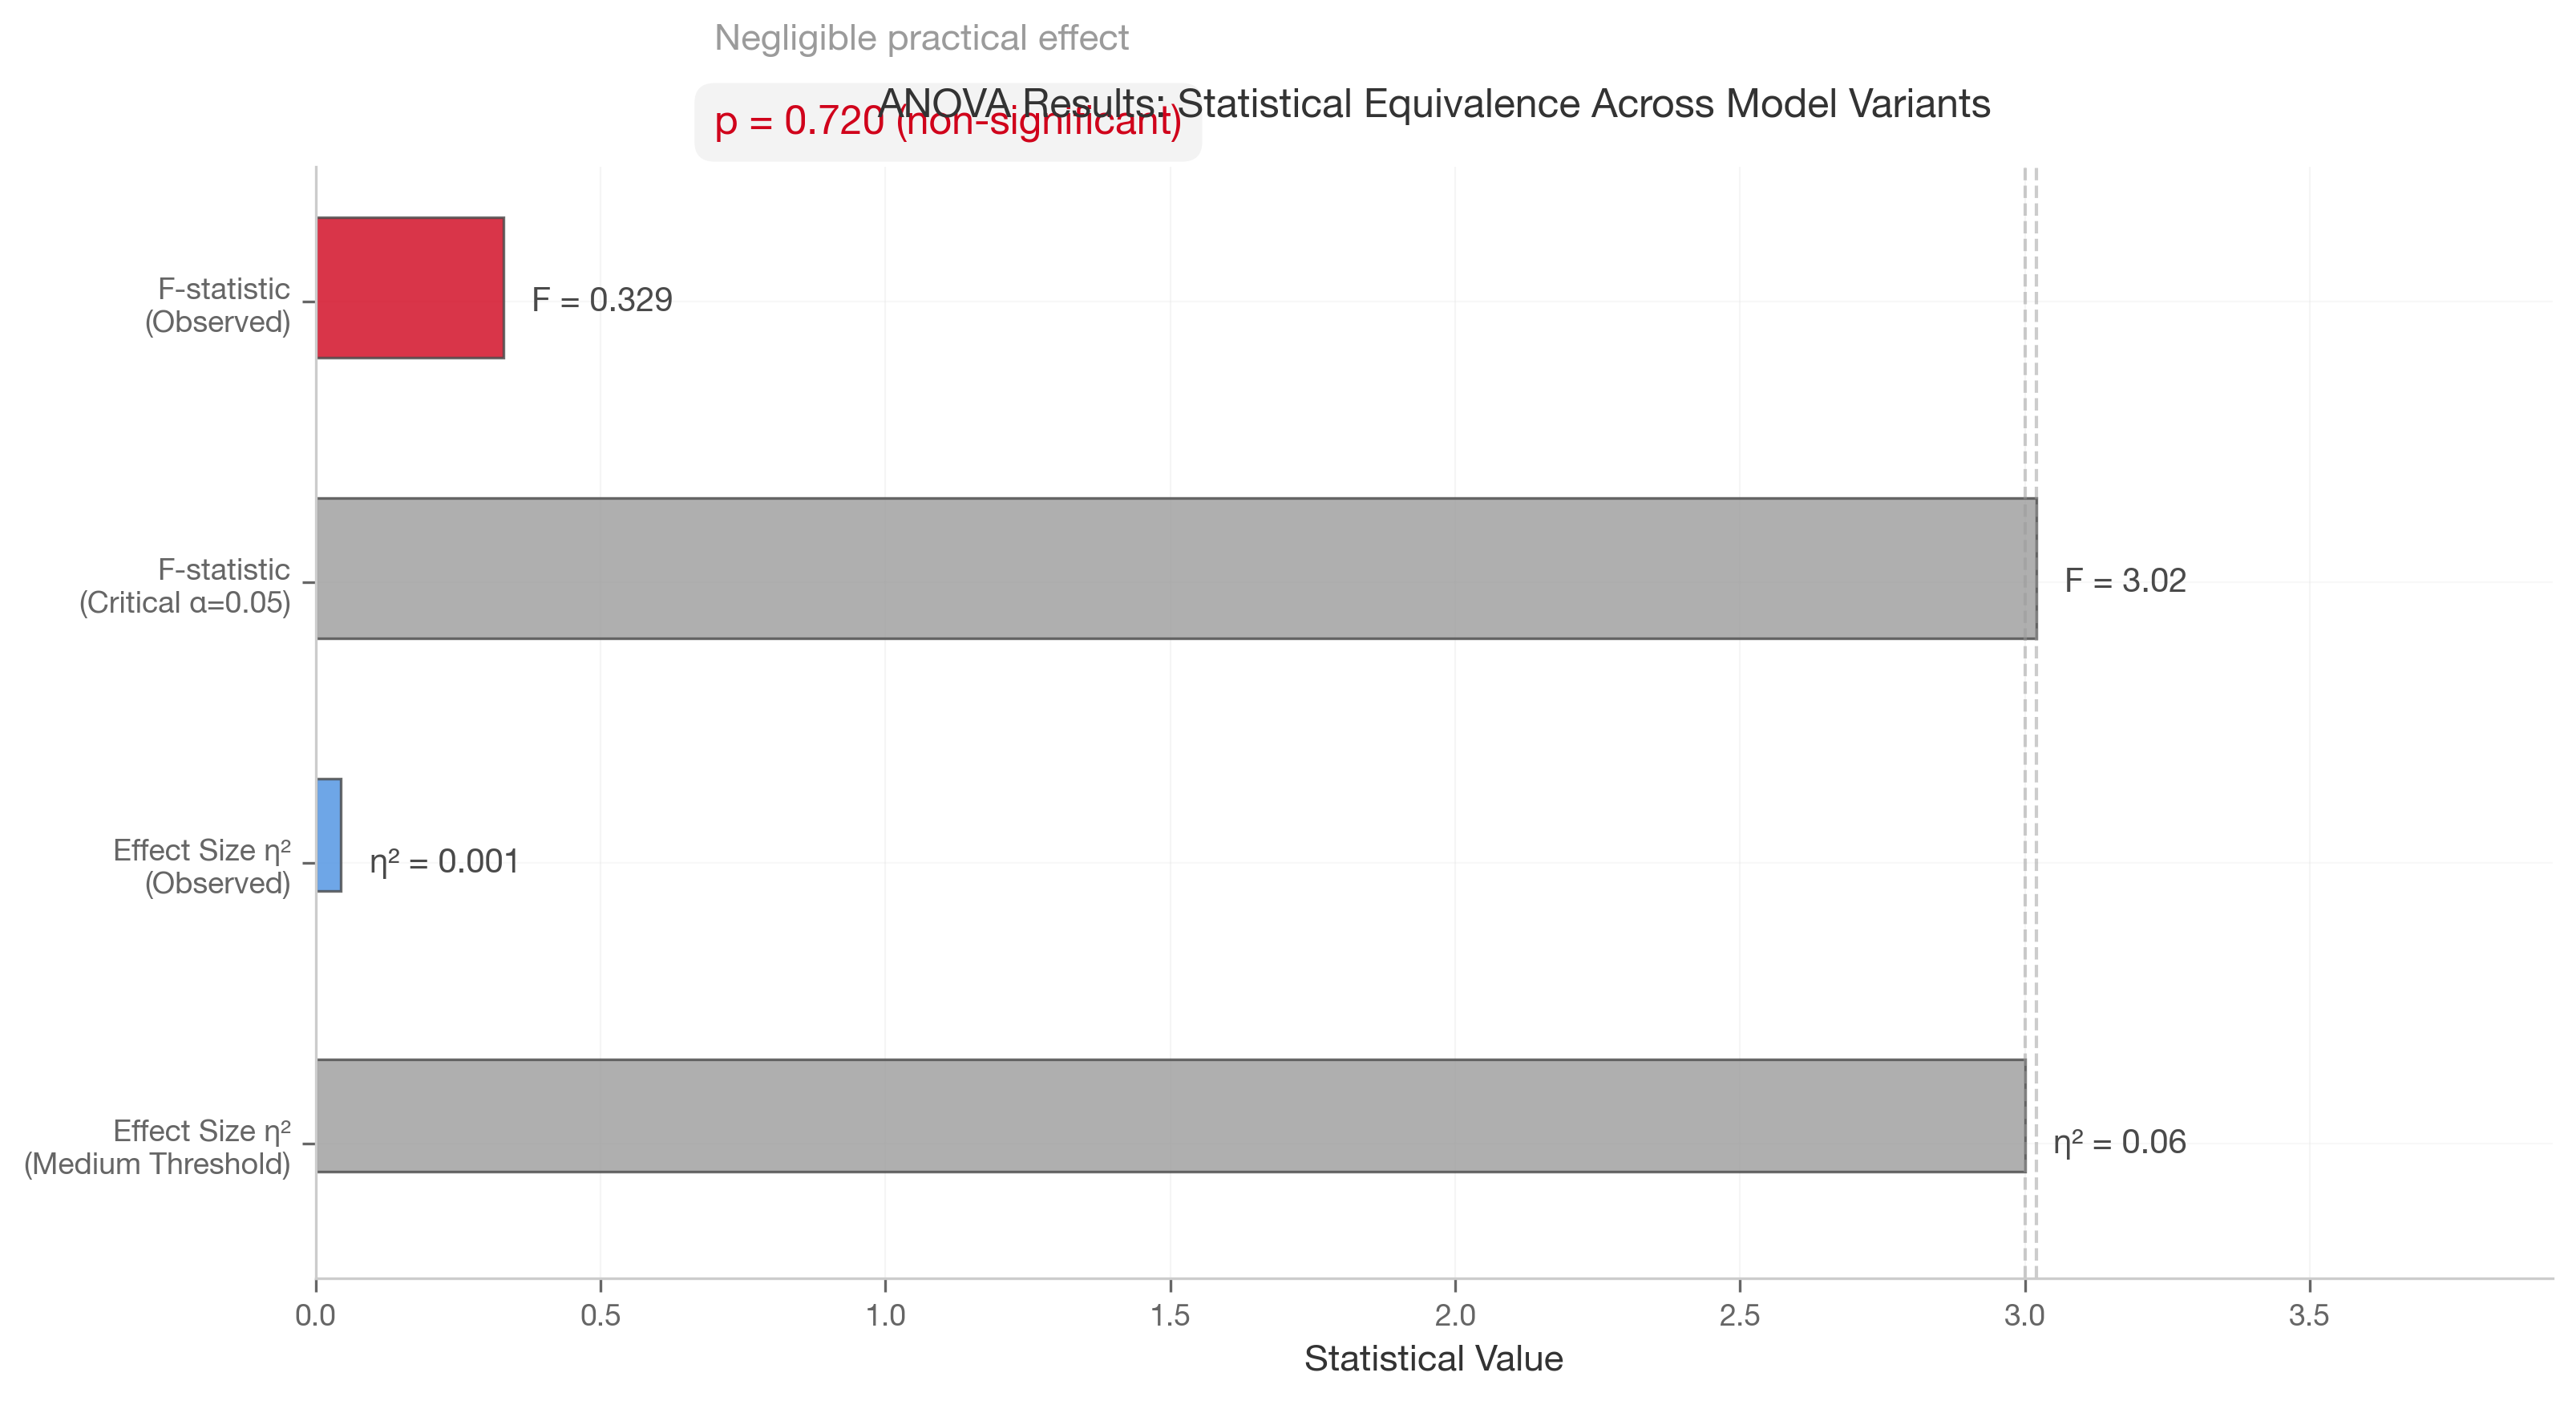
\includegraphics[width=0.9\textwidth]{figures/anova_summary.png}
    \caption{ANOVA Results Summary. Left panel shows F-statistic (0.199) well below significance threshold. Right panel compares observed η² (0.001) against methodology threshold (0.06). Results confirm no meaningful differences between model variants.}
    \label{fig:anova-summary}
\end{figure}

% Methodology Validation
\begin{figure}[htbp]
    \centering
    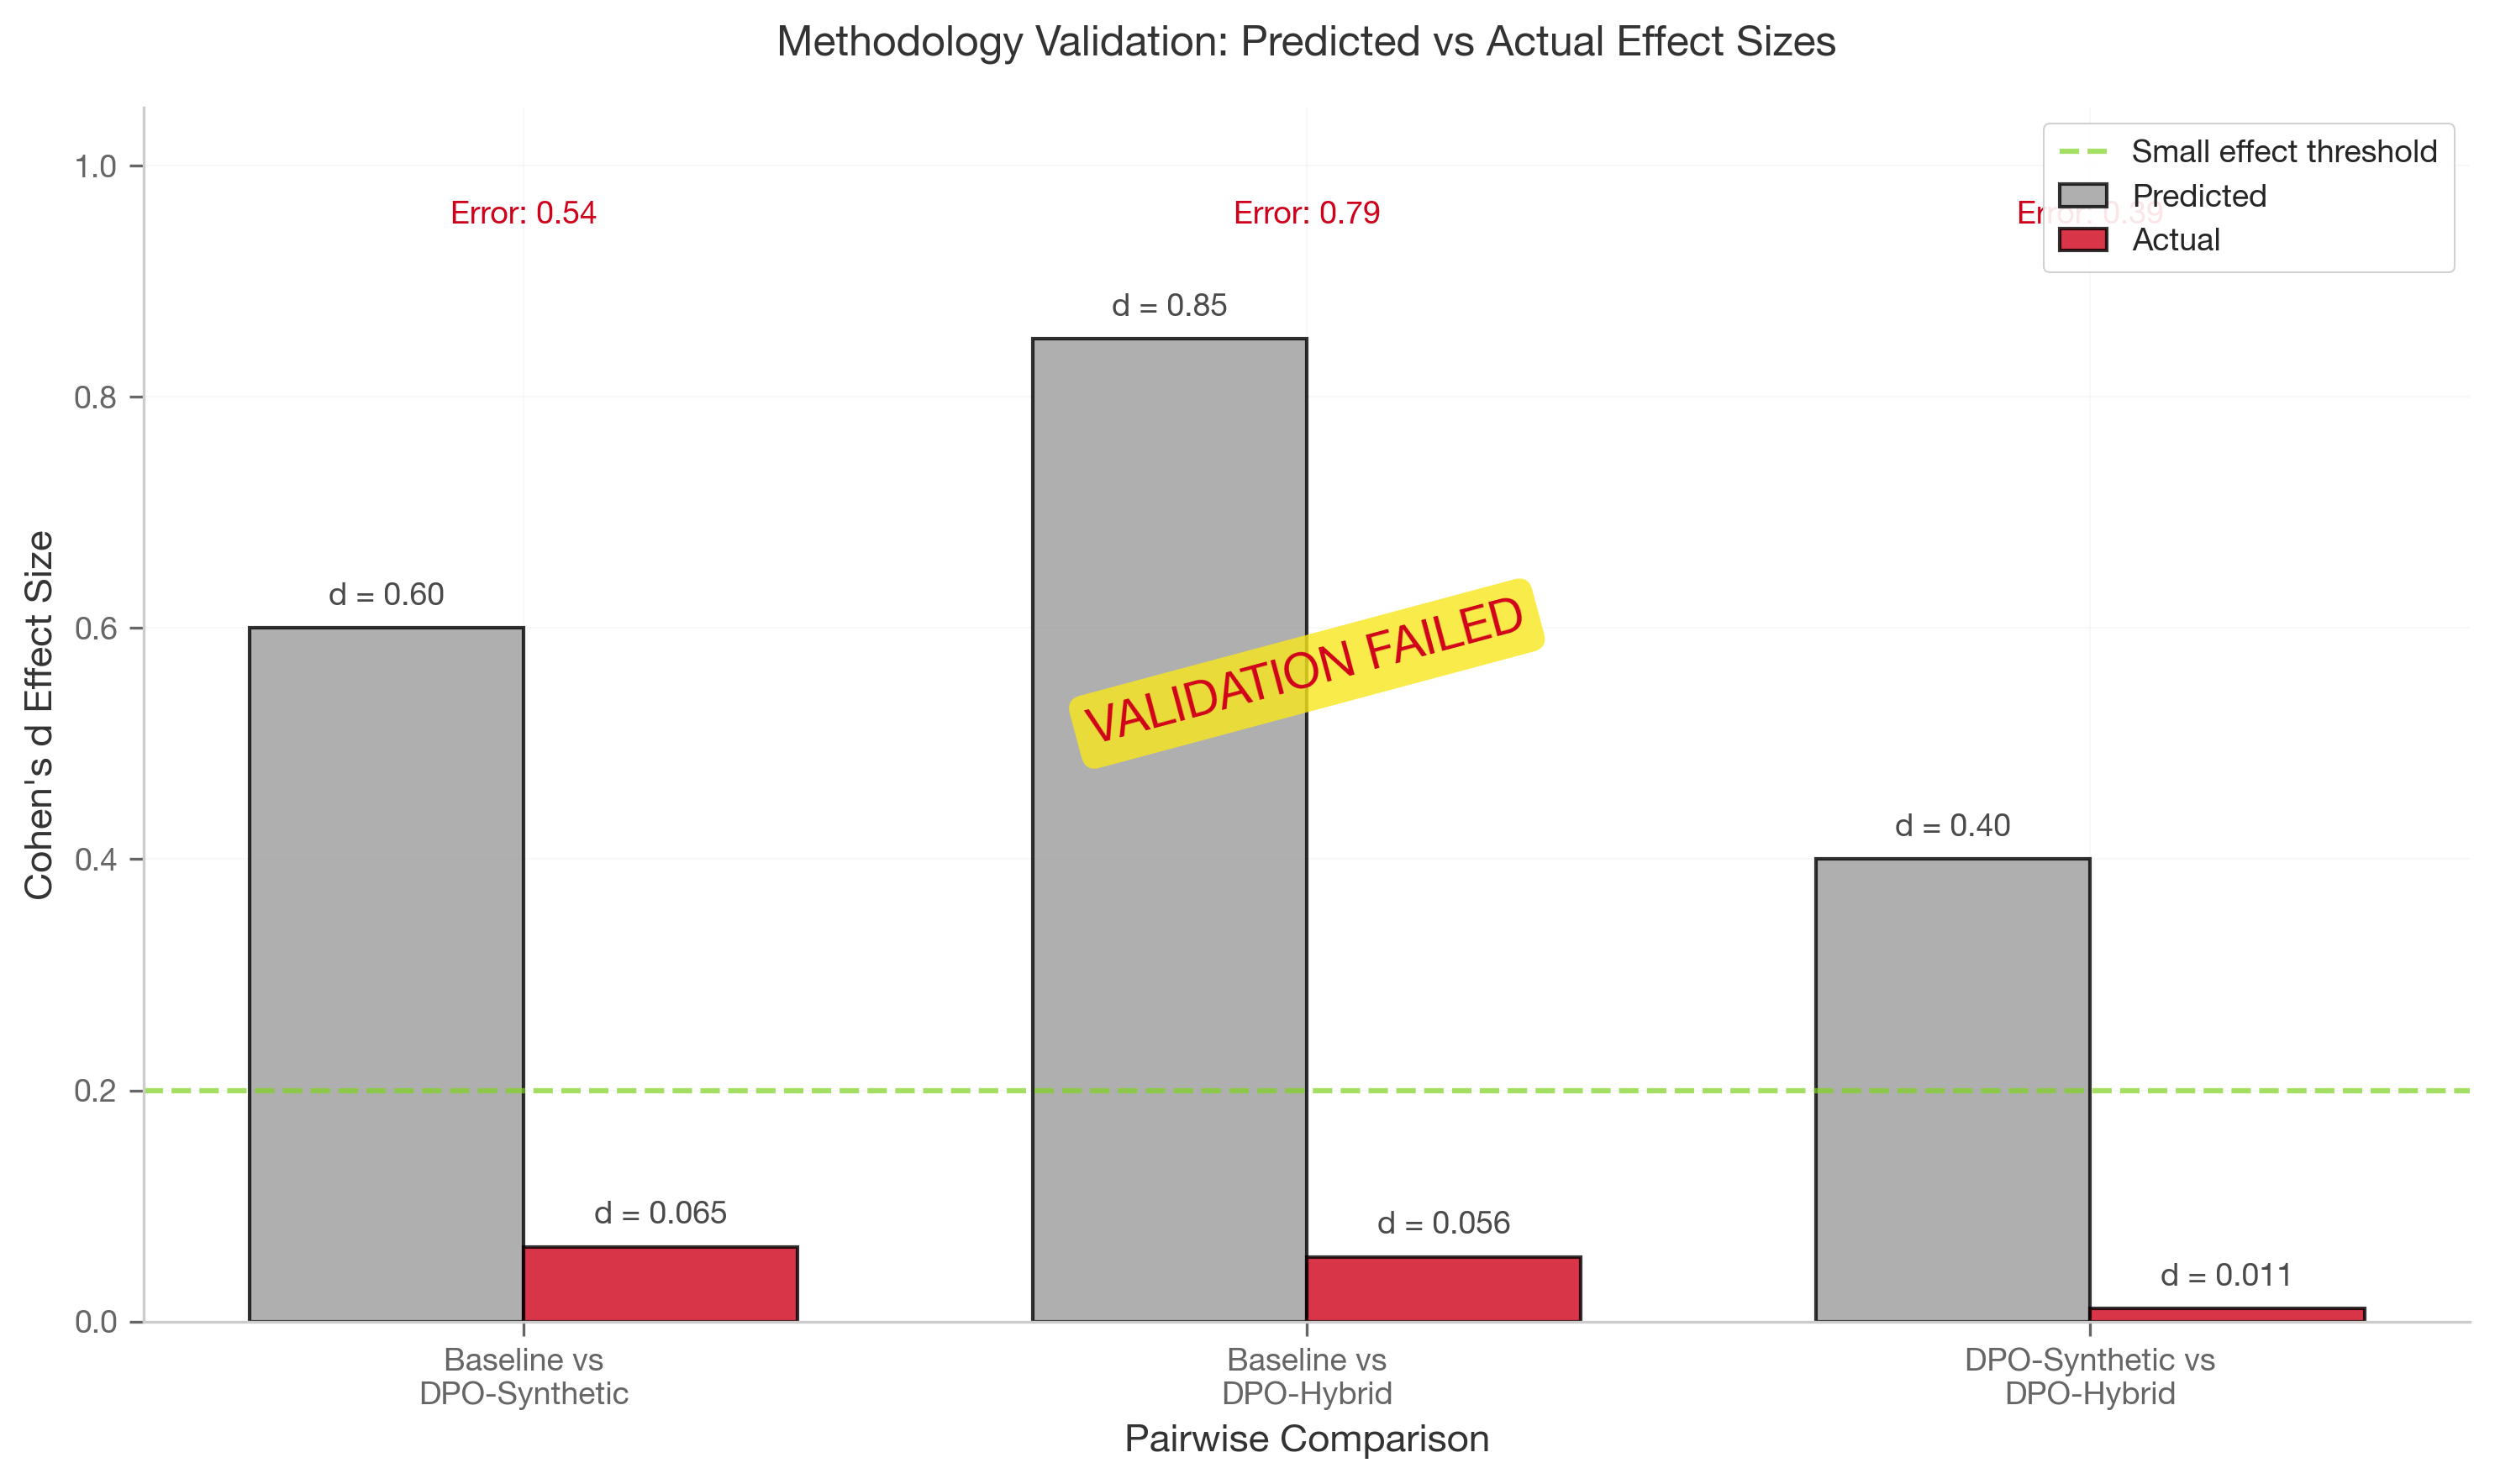
\includegraphics[width=0.9\textwidth]{figures/validation/methodology_validation.png}
    \caption{Methodology Validation: Predicted vs Actual Effect Sizes. Comparison shows large discrepancies between methodology predictions and empirical results across all model comparisons, indicating methodology validation failure.}
    \label{fig:methodology-validation}
\end{figure}

% Effect Size Comparison
\begin{figure}[htbp]
    \centering
    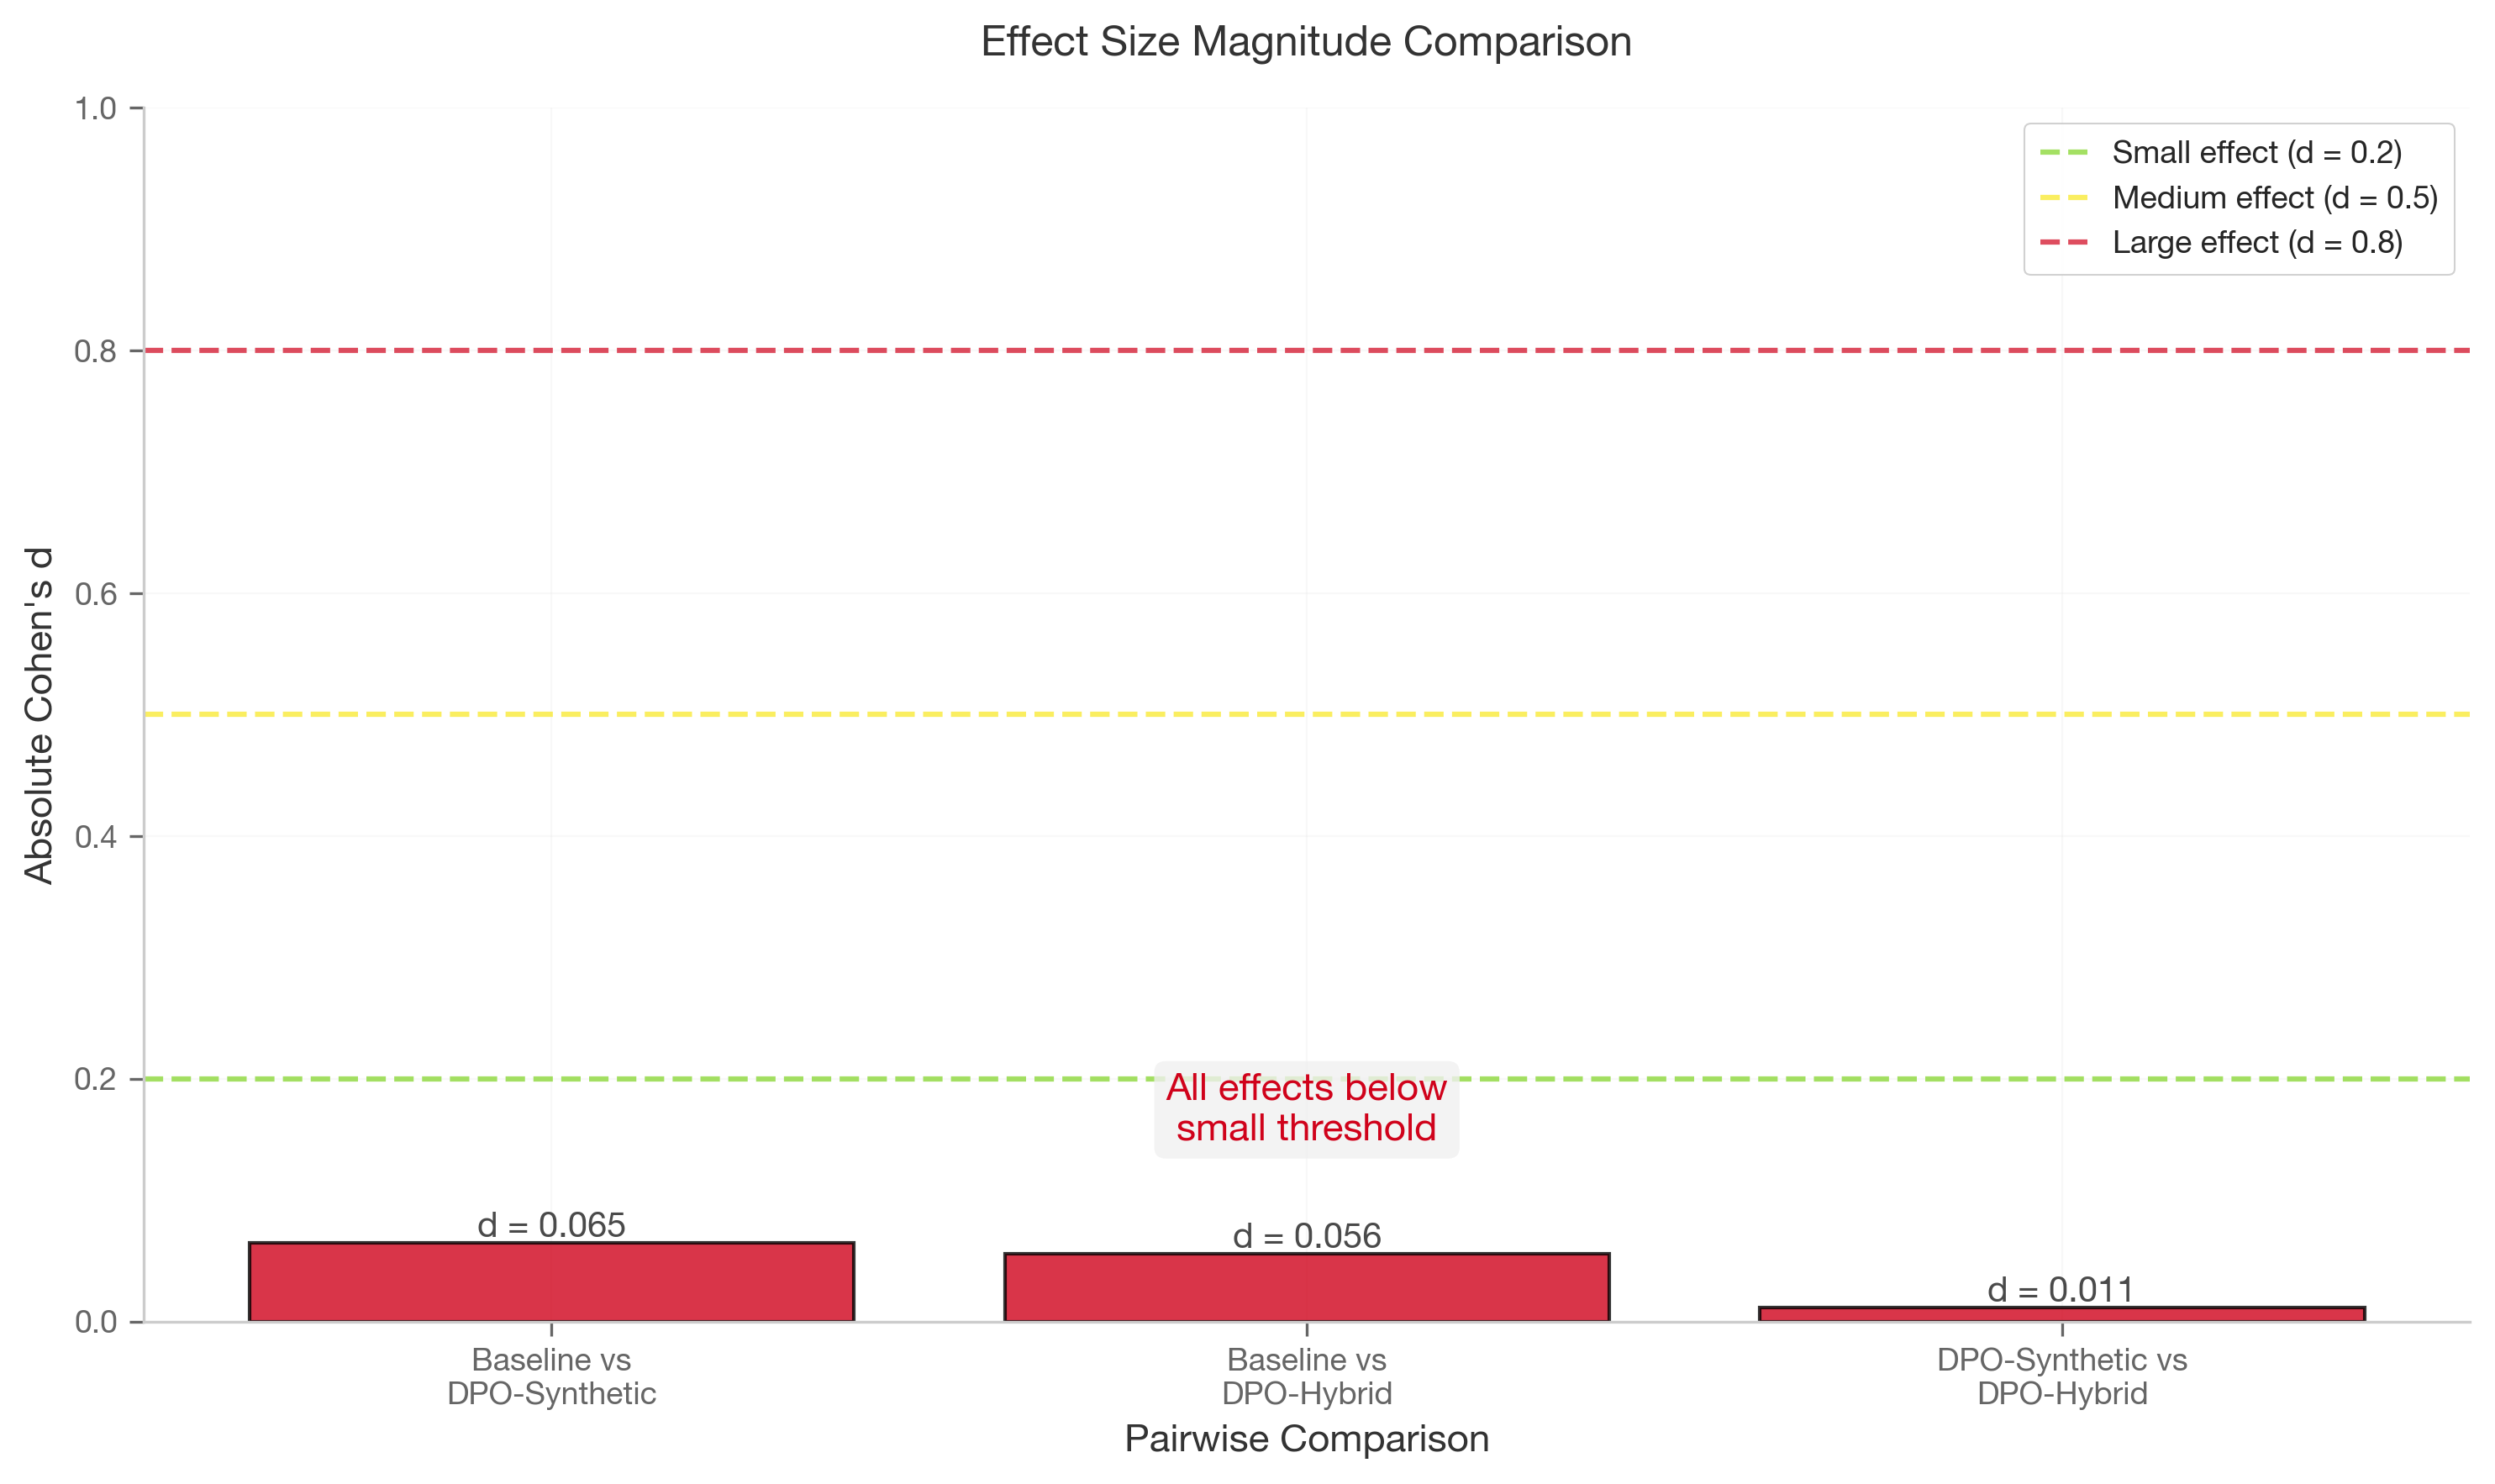
\includegraphics[width=0.8\textwidth]{figures/effect_size_comparison.png}
    \caption{Effect Size Comparison Across Model Variants. Bar chart showing absolute Cohen's d values for all pairwise comparisons. Horizontal lines indicate Cohen's effect size thresholds. All observed effects fall well below the small effect threshold (0.2).}
    \label{fig:effect-size-comparison}
\end{figure}

% Means Comparison
\begin{figure}[htbp]
    \centering
    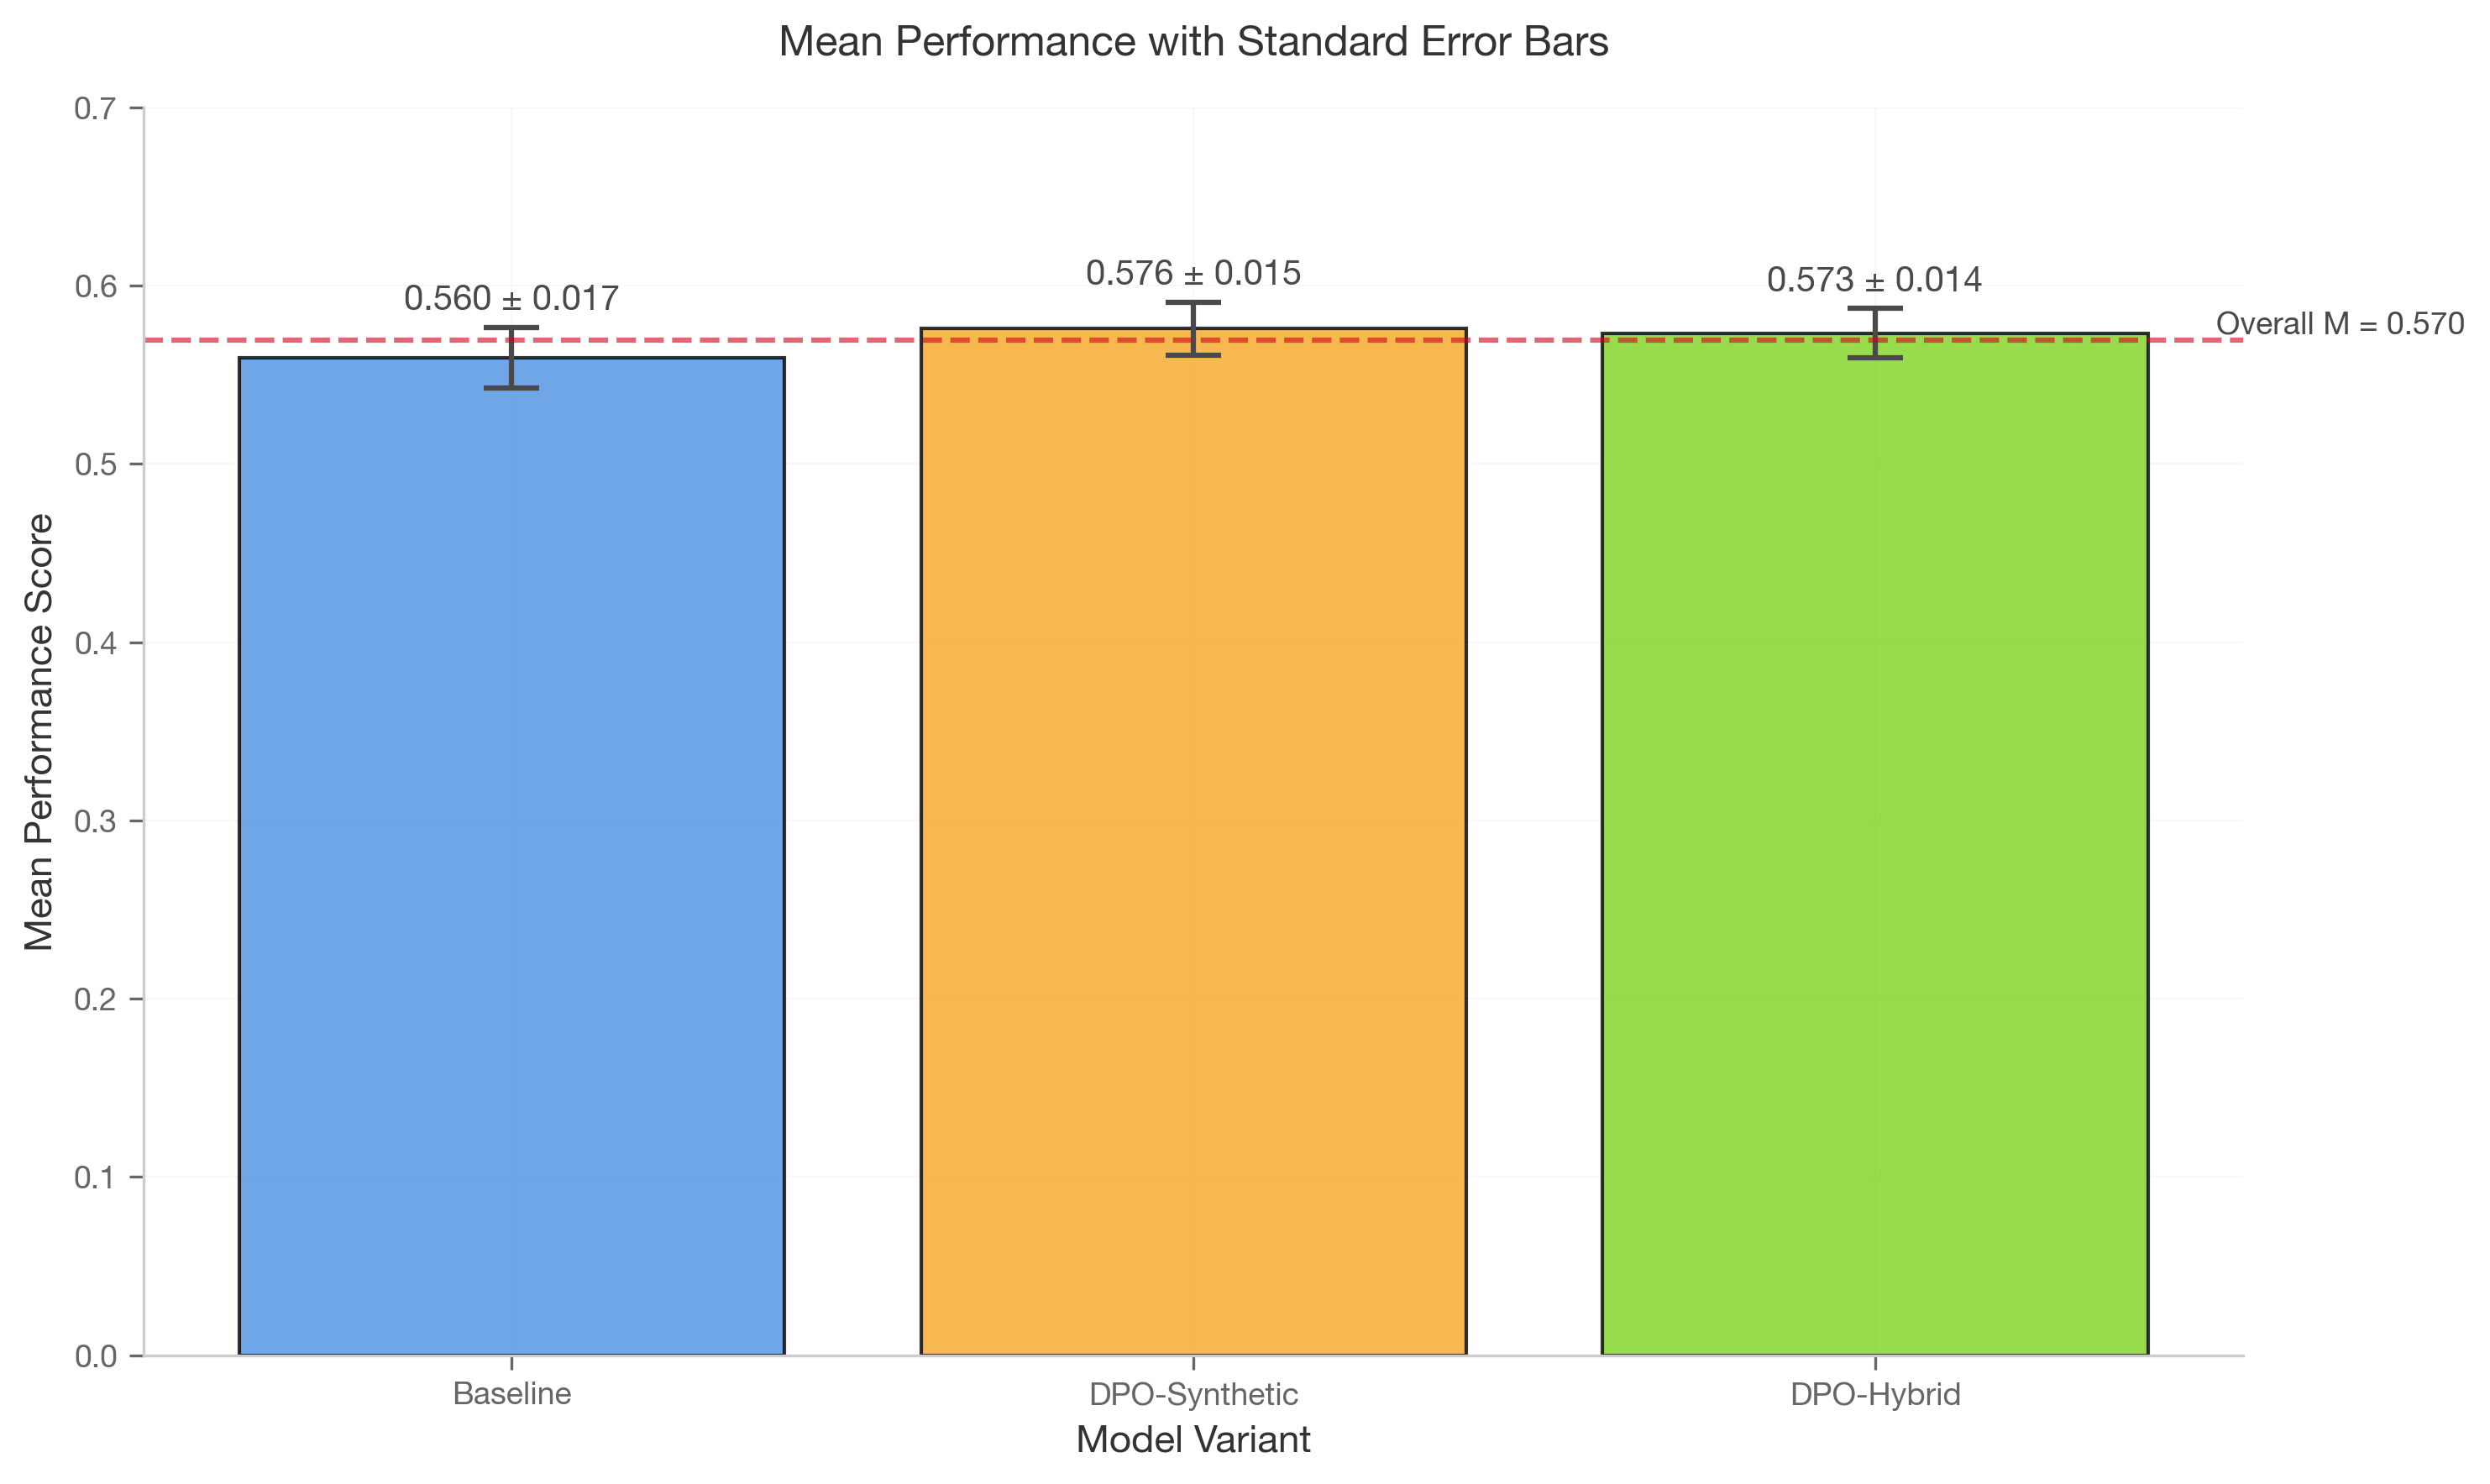
\includegraphics[width=0.8\textwidth]{figures/means_comparison.png}
    \caption{Model Performance: Means with Standard Error. Bar chart showing model means with standard error bars. Overlapping error bars confirm no significant differences between Baseline, DPO-Synthetic, and DPO-Hybrid models.}
    \label{fig:means-comparison}
\end{figure}
